Let $M=\llbracket 1,n \rrbracket$ the set of \emph{mainline link} indexes and $R\subset{M}$ the set of mainline link indexes whose exit node is connected to a ramp (i.e. the set of ramps, indexed by their preceding mainline link). \\
We denote as $T\subset{M}$ the set of monitored mainline links  (T for 'tracked') and $K=\{ i_{1},i_{2},...,i_{\kappa}\}\subset{R}$ the set of the $\kappa$ non-monitored ramps (K for "knobs").\\
$(L_{i})_{i\in M}$ are the lengths of the mainline links.\\
\begin{figure*}[t]
	\centering
	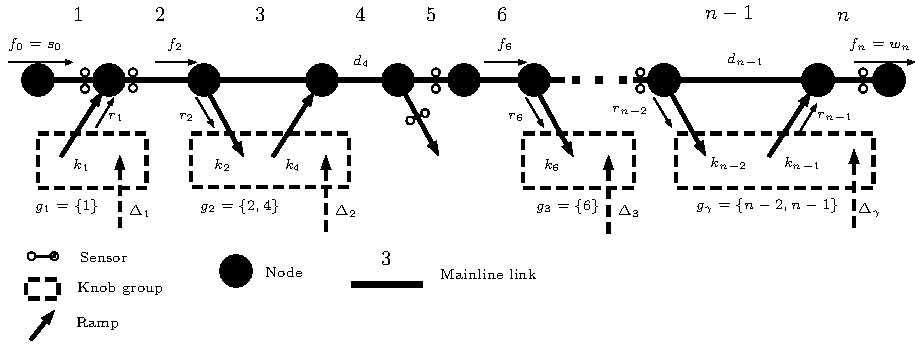
\includegraphics[width=7in]{figures/scheme.pdf}
%	\normalsize{
%		\begin{tabular}{llll}
%		\ \ \ \ \ \ \ \ \ \ \ \ \ \ && \ \ \ \ \ \ \ \ \ \ \ \ \ \ & \\ 
%
%			&$M=\llbracket 1,n \rrbracket$ && Mainline links indexes\\
%			&$S=\{ i_{1},i_{2},...,i_{s}\}\subset{M\cup\{0\}}$ && Source links indexes (index of preceding 	mainline link)\\
%			&$W=\{ i_{1},i_{2},...,i_{w}\}\subset{M}$ && Sink ("well") links indexes (index of preceding mainline link)\\
%			&$T=\{ i_{1},i_{2},...,i_{\mu}\}\subset{M}$ && Monitored (T for tracked) mainline links indexes\\
%			&$K=\{ i_{1},i_{2},...,i_{\kappa}\}\subset{S\cup W\backslash \{0,n\}}$ && Non-Monitored ramps indexes : the "knob ramps"\\
%			&$G=(g_{i})_{i\in{\llbracket 1,\gamma \rrbracket}}$ && Knob groups\\
%			&$k_{p}=(k_{i_{1}}^{(p)},k_{i_{2}}^{(p)}...,k_{i{\kappa}}^{(p)})$ && Knobs value vector at iteration p\\
%			&$\sigma=(\sigma_{i_{1}},\sigma_{i_{2}}...,\sigma_{i_{\kappa}})$ && $\pm1$ : on- or off-ramp indicator for knobs\\
%			&$(L_{i})_{i\in M}$ && Mainline link lenghts\\
%			&$(f^{(p)}_{i}(t))_{i\in{M}}$ && Mainline out flows at iteration p\\
%			&$(s^{(p)}_{i}(t))_{i\in{S}}$ && Source out flows at iteration p\\
%			&$(w^{(p)}_{i}(t))_{i\in{W}}$ && Sink out flows at iteration p\\
%			\\
%		\end{tabular}
%	}
	\rule{7in}{0.3pt}
	\caption{Freeway model and notation}
	\label{fig:scheme}
\end{figure*}
